\chapter{绪论}

\section{研究背景与意义}
基于位置的服务(Location Based Serve, LBS)不管是在工业还是民用领域都扮演着非常重要的角色,例如物流管理、航道规划、智慧交通、自动驾驶以及智能家居等\cite{iot-lbs}。在室外环境中,全球导航卫星系统(Global Navigation Satellite System, GNSS)诸如美国的GPS (Global Positioning System)以及中国的北斗卫星导航系统等都能够提供高精度低成本的定位服务,基本上满足了各种室外活动的需求。然而,在复杂多变的室内环境中,GNSS信号衰减严重导致定位精度下降,以至于很难满足室内定位的需求\cite{裴凌2017室内定位技术与应用综述,ips-gnss-mehrabian2023sensor}。近年来,物联网的飞速发展,一方面,室内环境如家庭、工厂以及商超等对位置服务有需求的终端设备数量指数级增长;另一方面,室内环境下对定位精度以及稳定性的要求也非常高。针对室内环境对位置服务在数量和质量上的需求,如何在复杂多变的室内环境下提供高精度、低成本以及稳定的位置服务是一个重要的挑战。

为了克服上述挑战,一些室内定位系统(Indoor Positioning System, IPS)被设计出来,它们利用各种不同的无线信源来发射信标,其中主要分为以下四类:射频信源、音频信源、磁源以及光源\cite{陈锐志2017基于智能手机的室内定位技术的发展现状和挑战,ips-wahab2022indoor}。

目前,使用射频信号的IPS种类最多,它们基本上都是工作在不同频段以及拥有不同的编码方案,如常见的蓝牙、WiFi (Wireless Fidelity)以及ZigBee、超带宽、蜂窝网络、伪卫星等\cite{闫大禹2019国内室内定位技术发展现状综述}。

其中,伪卫星通过地面基站发射类似GNSS信号来定位,优点是覆盖范围广,精度高,但是系统复杂和成本高昂\cite{李占营2018基于伪卫星技术的室内定位系统硬件设计及实现}。

蓝牙、ZigBee、WiFi、以及超带宽 (Ultra-wide-band, UWB) 四种方案,都是基于短距离无线通信技术,需要部署多个节点来覆盖室内所有区域,一般定位的精度跟信标节点的布局方式以及密度有关。其中,基于WiFi的IPS主要是通过指纹法和测距法来实现定位\cite{wifi}。测距法通过将不同信标节点的接收信号强度(Received Signal Strength, RSS)转化为距离来估计接收端的位置,这种方法相对于指纹法不需要建立和维护指纹数据库并且拥有更高的精度,但是由于室内环境的复杂多变,因此很难进行准确的信道建模,从而无法准确的构建信号强度与距离之间的关系。随着IEEE802.11标准的更新,增加了通过计算接收端与信标节点之间的报文时间戳来估算信标节点到接收端的时间,从而估计两者之间的距离,这种方法不需要对信道进行建模,但是对时间同步有很高的要求。基于蓝牙的IPS和基于WiFi的IPS类似,都可以通过指纹法和测距法来实现定位\cite{bluetooth}。此外,在蓝牙5.1协议中增加了方向测量的方案,补充了通过多天线阵列的信号相差来测量离开角度和到达角度的功能,因此基于蓝牙5.1的IPS系统可以使用到达角度 (Angle of Arrival, AOA)来定位。基于蓝牙的IPS拥有低功耗、低成本的优点,但是通信距离短导致需要更密集的信标节点。为了增加通信距离需要提高广播信道的功率。基于ZigBee的IPS主要是通过指纹法来进行定位,拥有低成本、低功耗等优点。然而,由于IEEE 802.15.4标准低速率、大延迟的缺点,基于ZigBee的IPS更容易受到噪声的干扰以及多径效应的影响导致定位精度下降,并且很难满足实时定位的要求\cite{ZigBee}。UWB由于其高带宽的特点拥有非常高的传输速率,又因为发送的是窄脉冲的数据包,因此拥有很高的时间分辨率\cite{uwb}。因此,基于UWB信号的IPS通过使用TOA (Time of Arrival, TOA)的定位方法可以获得非常高的精度。然而,由于极高的时间分辨率,将导致在非视距下的信号延迟可能使系统无法正常工作。除此之外,也可以通过部署多个UWB节点来测量到达角度,从而使用AOA定位方法。UWB定位拥有非常高的精度以及速度,但是成本也非常高。

基于蜂窝网络的IPS通过主要是通过邻近匹配法来判断接收端到附近基站的位置\cite{LTE}。作为最新的蜂窝移动通信技术,5G(毫米波)技术的大带宽和大规模天线阵列带来了更高的通信速率和更低的延迟,一方面可以提高基于TOA技术的定位精度,另外一面,大规模天线阵列可以提高角度测量的精度从而提高基于AOA定位方法的精度。除此之外,高频信号和低延迟更有助于抵抗多径效应。然而,基于蜂窝网络的IPS主要的挑战是定位精度、成本与基站密度的问题。基于5G技术的IPS拥有很高的定位性能与5G基站的密集程度有关,但是更高的功耗以及建造成本也不容忽视\cite{5g}。

使用音频信号的IPS根据音频的波段分为超声波定位和音频定位,都是通过计算时间来估计距离,前者是计算超声波经过反射回到出发点的时间\cite{室内超声波定位系统},后者计算的是声音从基站到达接收端的时间\cite{曹帅2020面向智能移动终端的音频室内定位关键技术研究}。由于声音的传播速度相较于电磁波非常慢,因此对时间同步的精度要求不高,但是受多径效应和非视距的影响非常严重。并且,由于超声波频率容易受到温度影响,因此对待定位设备所处的环境以及其数量有要求,总体来说,系统复杂成本较高。音频定位由于工作频率在人耳可听的范围内,环境声音可能会对其造成干扰。

利用磁源进行室内定位的有两种主流方案,第一种是利用地球磁场进行定位,另外一种是认为铺设磁源设备进行定位。前者根据地球磁场在地理位置上的差异性来构建指纹数据库,接收端可以根据采集到的磁场强度的方向来匹配指纹库从而判断自己的位置。但是由于室内环境中小范围的磁场差异不明显导致定位误差较大。因此,在很多物流场地,通过人为在地面铺设磁源设备来增加区域的磁场差异性,从而提高定位精度。同样的,定位精度取决于磁源设备的密集程度\cite{周家鹏2019地磁室内定位技术研究,ips-wang2023improved}。

根据光的波长可以将基于光源信号的IPS分为红外线定位和可见光定位(Visible Light Positioning, VLP)。红外线定位首先待定位物体通过周期性的发送的包含特殊标记的红外信号给探测器,探测器在探测到红外信号后将自己的信息发给服务器,服务器从而知道带定位物体的位置,这种定位方法其实也是邻近匹配法,定位精度不高,目前很少使用。

VLP作为一种最新的室内定位方法,通过可见光通信(Visible Light Communication, VLC)技术来实现对信标的接收\cite{vlp-abdalmajeed2023improved,vlp-sen20233d}。首先,发送端通过对位置坐标进行编码然后按照一定的调制方案来驱动发光二极管(Light Emitting Diode, LED)发送调制光信号,接收端通过光电探测器 (Photo-diode, PD) 或者图像传感器(Image Sensor, IS)捕捉随时间变化的光强度信号\cite{ips-pd-is-liu2022efficient}。通过解调解码来获取发送端的坐标,与此同时,通过接收到的信号强度估计接收端和发送端之间的几何关系,从而估计自身的位置。VLP凭借下述的优越性,在IPS中非常具有潜力:
\begin{enumerate}[topsep = 0 pt, itemsep= 0 pt, parsep=0pt, partopsep=0pt, leftmargin=20pt, itemindent=0pt, labelsep=6pt, label={(\arabic*)}] 

    \item 可见光的频谱非常宽,因此VLC拥有无限制的频谱资源。这对于基于射频信号以及音频信号的IPS来说,非常的关键。考虑到物联网的快速增长,频谱资源日益紧张,当海量终端同时运行时,可能存在竞争频谱资源导致的通信阻塞、链路中断等问题。
    \item 部署更多信源节点的成本很低。由于LED工艺的发展,LED造价低、功耗低、寿命长,安装简单,相对于其他IPS来说,将不再考虑由于部署更多节点带来的成本问题,因而VLP系统的成本可以控制在非常低的一个水平。
    \item VLP在物理层有更高的安全级别。由于可见光直接视距(Line-of-sight, LOS)传播特性,将保证物理层信号不容易被监听。
    \item VLP系统的定位精度非常高。在目前已经实现的很多VLP系统中,可以实现低成本的同时具有很高的定位精度。
\end{enumerate}

表\ref{tab:positioning-systems} 总结了目前主要的一些IPS的定位方法以及优缺点。考虑到VLP在频谱资源、成本以及定位精度等方面与基于射频信源、音频信源以及磁源的IPS有很大的优越性,我们认为室内VLP系统在复杂多变的室内环境下提供高精度、低成本以及稳定的位置服务最有潜力。
\begin{table*}[!htbp]
  \centering 
  \small
  \caption{不同类型的室内定位系统对比}  
  \label{tab:positioning-systems}  
  \begin{tabularx}{\textwidth}{lccc}
    \toprule
   \textbf{信源类型}   &   \textbf{定位方法}     & \textbf{优点}     &\textbf{缺点} \\
    \midrule
    伪卫星    &   TOA   &   精度高,覆盖范围广    &     系统复杂,成本高昂  \\
    
    WiFi    &   RSS测距   &   功耗低,易部署  & 信道建模比较复杂,影响精度  \\
    WiFi    &   TOA   &   功耗低,易部署  & 时间同步要求高  \\

    蓝牙    &   AOA   &   成本低,功耗低,易部署  & 覆盖范围小,需要密集部署  \\
    
    ZigBee    &   指纹对比   &   成本低,功耗低   &  易受噪声和多径的影响,实时性低  \\
    
    超带宽    &   TOA   &   精度高    &成本高,受非视距影响严重  \\
    
   蜂窝网络    &   邻近匹配   &   简单,易实现    &精度低,受多径影响  \\
   
   5G毫米波    &   TOA、AOA   &   精度高,抗多径干扰    &成本高  \\

   音频    &   TOA、TDOA   &   成本低,易部署    &受多径和环境声影响  \\
   
   磁场 &   指纹匹配   &不受遮挡的影响       &建立和维护指纹库成本高  \\
   
   可见光 &   TDOA、CV   &精度高、成本低       &受非视距影响  \\
   
    \bottomrule
  \end{tabularx}%
\end{table*}%



\section{研究现状与挑战}
\subsection{可见光通信的研究现状}
VLC是一种通过对频率在400-800THz的可见光进行调制来传输数据的通信技术,凭借其安全、无电磁辐射、免频谱授权等优点,是最有潜力的下一代无线通信技术之一\cite{vlc-sejan2023comprehensive}。可见光波谱如图\ref{fig:spectrum}所示,远大于无线电频谱。
\begin{figure*}[!htbp]
  \centering
  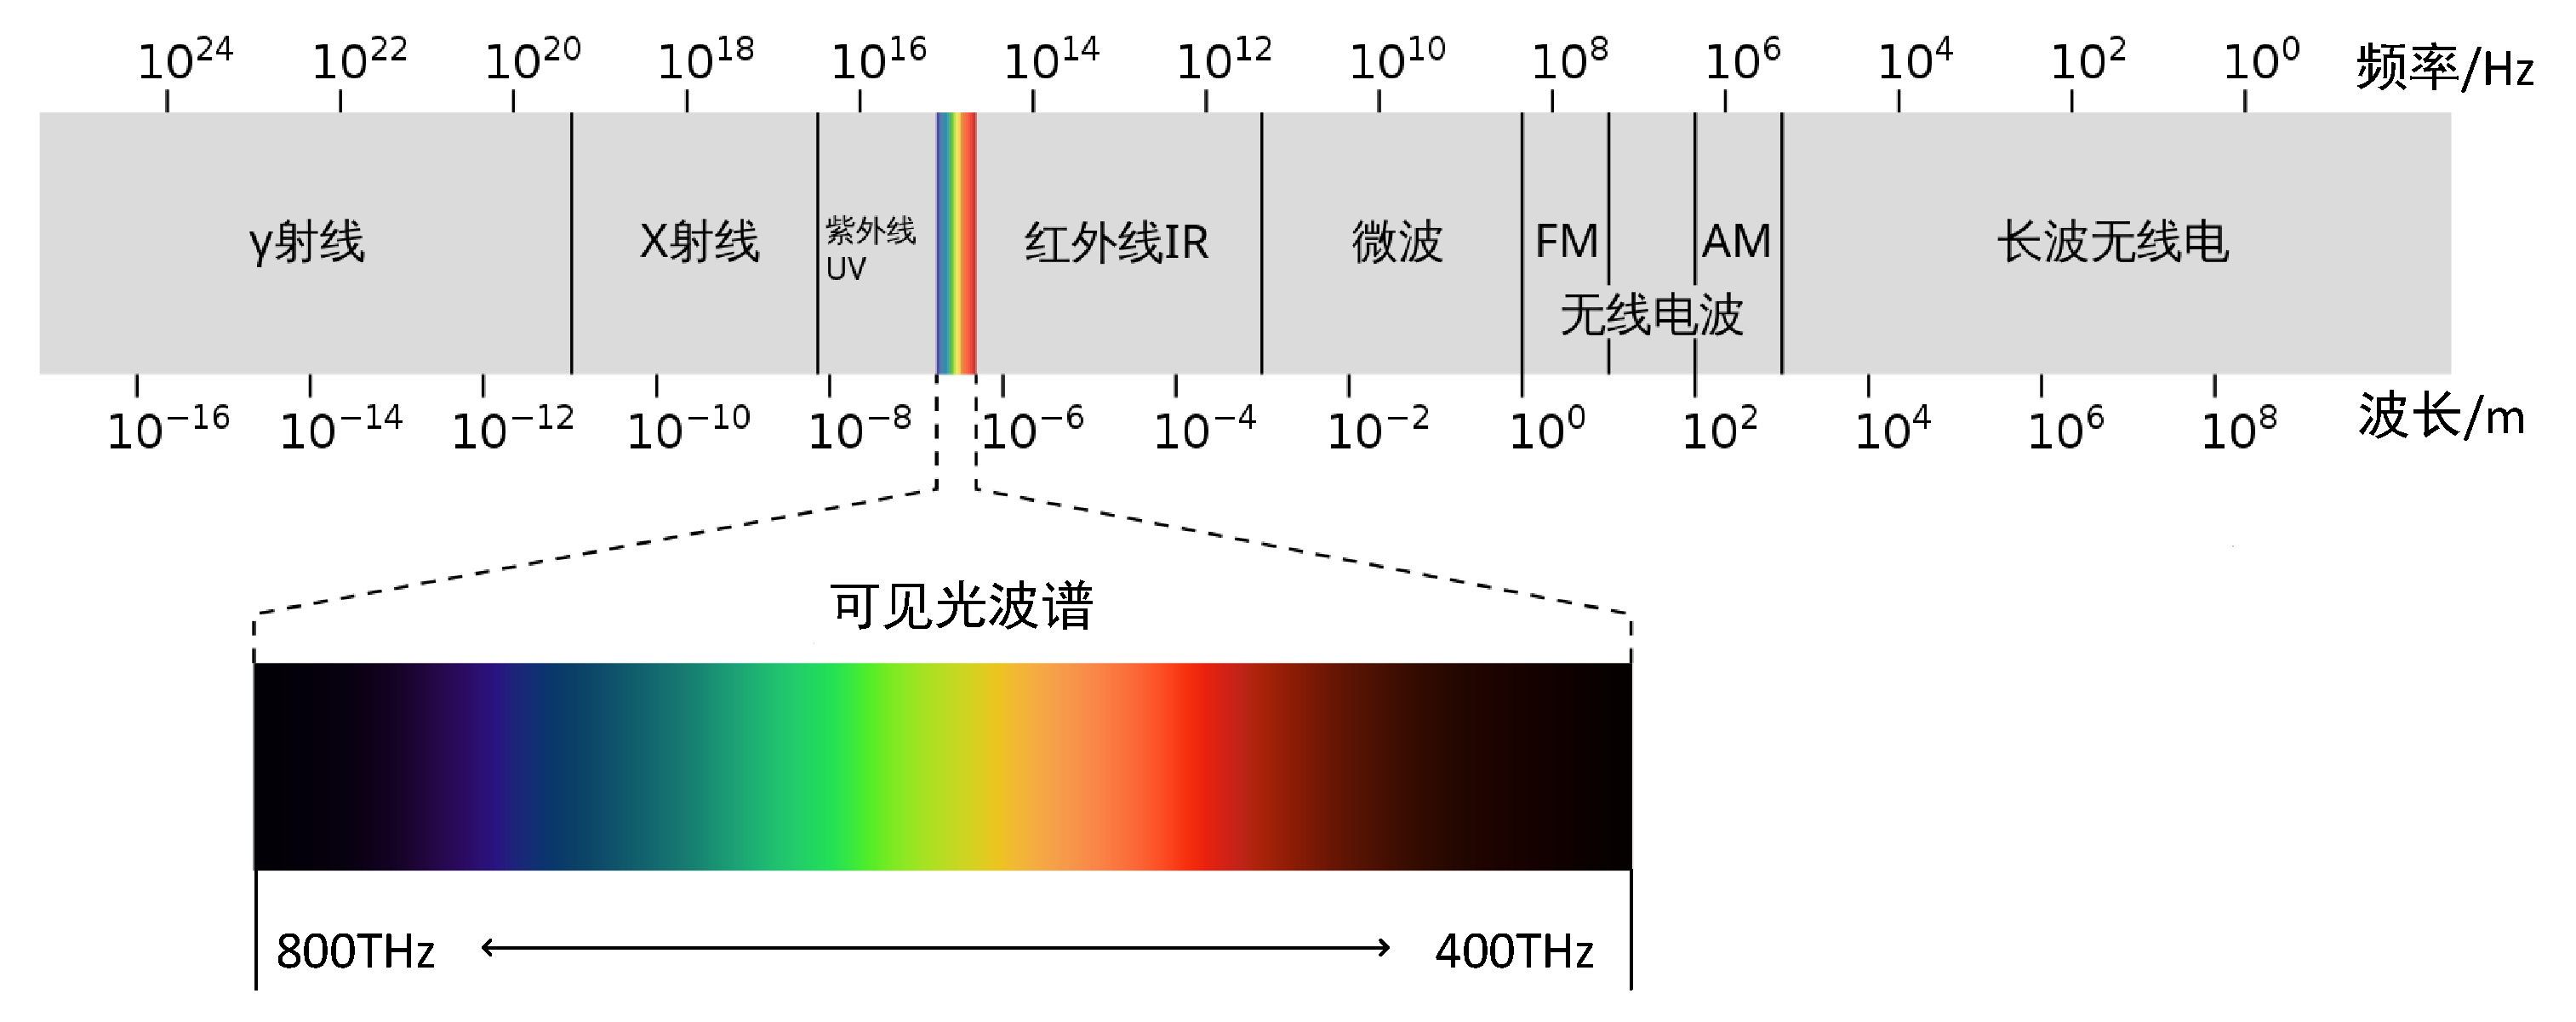
\includegraphics[width=\linewidth]{FIG/Eletornic spectrum.pdf}
  \caption{可见光波普}
  \label{fig:spectrum}
\end{figure*}


虽然古代军事上早就应用了VLC来传输信息,但是现代意义上的VLC概念最早是在1999年由香港大学G.Pang教授提出来的\cite{1211-vlc1999}, G.Pang教授在实验中利用VLC技术实现音频信号传输。

2000,日本中川实验室Tanaka等人提出使用白色LED的照明设备应用于无线家庭链路中的接入点,并通过仿真验证了该方案的可行性\cite{1212-vlc2000}。随即,日本研究人员开始意识到VLC的潜力以及存在的巨大应用前景,相应的,日本政府在2003年的时候成立了“可见光通信协会 ”,旨在助力VLC系统产业化。2004年,日本学者Komine等人讨论了干涉和反射对VLC系统的影响,对VLC信道研究奠定了理论基础\cite{1213-vlc2004}。

在之后的几年时间里,大量学者对VLC系统进行了研究,VLC系统的通信速率从几kbps快速发展到了几十Mbps,特别是2009年英国牛津大学的Minh等人考虑到了普通白光LED有限带宽对VLC速率的限制,通过蓝色滤波结合简单的接收机均衡,可以实现50MHz的带宽和100Mbps基于开关键控不归零调制的数据链路\cite{1214-vlc2009}。与此同时,欧洲政府开始启动1Gbps VLC系统研究项目,将VLC技术是为家庭无线接入技术的重要研究对象。由于VLC的快速发展,IEEE于2011年发布了关于VLC的IEEE 802.15.7协议,该协议作为第一个VLC国际标准,定义了用于VLC的PHY层和介质访问控制层,并承诺了足以支持音频和视频多媒体服务的数据速率。同年,英国爱丁堡大学数字通信研究中心的Harald Hass 教授提出了LiFi (Light-fidelity) 的概念,认为VLC可以做到低功耗的同时实现1Gbps以上的高速通信\cite{1215-vlc2011}。

然而,硬件的性能以及传统的调制方式限制了高速VLC的发展。为了提高VLC的速率,一方面,大量的工作开始研究发射端、接收端的硬件性能,包括发射端器件如RGB-LED、磷光LED、硅基LED(Si-LED)、micro-LEDs阵列以及微型激光二极管(Laser Detector, LD)等等\cite{1216-vlc-rgb,1217-vlc-blue-led,1218-vlc-si-led,1219-vlc-microled,12110-vlc-ld},和接收端光电探测器如PIN阵列、微型探测器阵列(Micro-photo-detector, μPD)、雪崩式光电二极管(Avalanche Photo-diode, APD)、单光子雪崩二极管(Single-photon Avalanche Diode, SPAD)等\cite{12111-vlc-pin,12115-vls-upds,12112-vlc-apd,12114-vlc-spad,12113-vlc-spad}。另外一方面,针对VLC先进调制技术的研究也非常多,包括波分复用(Wave Division Multiplexing, WDM),正交频分复用(Orthogonal Frequency Division Multiplexing, OFDM),无载波幅度相位调制(Carrier-less Amplitude and Phase, CAP)和离散多音(Discrete Multi-tone, DMT)等\cite{12116-vlc-wdm,12117-vlc-ofdm,12118-vlc-ofdm,12119-vlc-cap,12120-vlc-cap,12121-vlc-cap,12122-vlc-dmt}。近十年,通过使用高性能的器件和先进的调制技术,国内外大量的VLC研究工作表示取得了几Gbps到几十Gbps的通信速率,例如英国爱丁堡大学数字通信研究所LiFi研发中心在2017年通过紫光微型LED阵列实现了11.95Gbps的数据传输速率\cite{12123-vlc-11.95G},该研究所在2019年通过WDM和OFDM结合,使用低成本的LED实现了15.73Gbps的通信速率\cite{12124-vlc-15.73G}。英国牛津大学工程科学学院在2018年提出了一个四色多路复用高速VLC系统,基于激光二极管的白光通信链路和宽视场角覆盖,实现了35Gbps的通信速率\cite{vlc-nature-35Gb}。我国科研院所在高速VLC系统的设计研发上也取得了很多重要成果,其中复旦大学迟楠教授团队在2015年通过WDM和CAP调制最早实现了VLC系统达到8Gbps以上速率\cite{vlc-chinan-8Gb},在2020年通过硅基多色LED阵列实现了20.09Gbps速率的领先水平\cite{vlc-chinan-20.09Gb},在2022年使用GaN超级发光二极管(Super Laser Detector, SLD),在国际上率先实现了在单芯片传输速率达到4.57Gbps的速率\cite{vlc-chinan-4.57Gb}。

IEEE 802.15.7协议规定VLC被作为一种短距离通信技术,大量的VLC实验演示系统通信距离都在几十厘米到几米的距离。虽然通过使用激光发射器作为发射端可以实现几十公里的通信距离,但是由于激光链路在远距离对准上的问题,只能应用在一些特定场合,并且由于覆盖范围较小,很难作为一种大规模商用的无线接入方案。目前在使用LED作为发射端的自由空间VLC系统中,复旦大学信息科学与技术学院电光源研究所设计了一种基于多色串联LED阵列的VLC系统,实验结果表明,在15.78Gbps的速率下实现了最远13m的远距离通信\cite{vlc-longdistance-13m}。值得注意的是,这是到目前为止基于LED的VLC系统所能达到的最远通信距离。

大量研究高速远距离VLC系统的工作为VLC的应用推广奠定了理论基础。与此同时,一些学者开始考虑将VLC技术应用于如智慧交通\cite{vlc-v2x-1,vlc-v2x-2}、室内VLP\cite{vlc-vlp-1,vlc-vlp-2}、水下可见光通信\cite{vlc-uwoc}等等场景。除此之外,考虑到相机在商业市场的普及程度,2012年英国爱丁堡大学的研究人员首次使用智能手机摄像头为接收端的VLC系统,实现了最大3.1Kbps的通信速率\cite{vlc-occ-first2012}。此后,这种为以相机为接收端的VLC被称为光学相机通信(Optical Camera Communication, OCC),开始受到了大量的关注\cite{vlc-occ,vlc-occ-2}。OCC系统通信速率与相机帧率正相关,目前已知的OCC系统可以做到的最高的通信速率是44.03kbps \cite{vlc-occ-5}。

虽然大量的研究工作在积极的推广VLC,但是VLC距离实用化还存在一定的距离,这主要是因为VLC面临几个主要的挑战,如LED的非线性、环境光干扰、上行链路以及视距等\cite{vlc-challenges}。其中,最主要的挑战是LOS受阻,在这种情况下,系统可能无法工作。目前,比较好的解决方法是通过反射光来进行通信,这种被称为非视距(Non-line-of-sight, NLOS) VLC。由于反射光信号的低信噪比,图像传感器在抗噪方面的特性由于PD,因此NLOS OCC受到更多的关注,特别是英国诺桑比亚大学Ghassemlooy教授团队在此方向上做了大量的工作\cite{vlc-nlos-1,vlc-nlos-2}。


\subsection{可见光定位的研究现状}
VLP是一种基于VLC的室内定位技术,通用的架构一般是通过调制驱动LED来发送包含位置信息的光信号,使用被固定在待测物体上的接收端来捕捉光信号,通过解调解码技术来获得LED的位置,然后使用位置估计算法来判断接收端的位置。

日本庆应义塾大学的M.Yoshino和C.Sertthin等人最早开始VLP的研究,2007年M.Yoshino等人基于VLC技术,通过使用IS和LED实现了定位\cite{is-first-1,is-first-2};2008年,C.Sertthin等人通过使用VLC技术来发送LED的位置信息,然后对接收端进行位置估算\cite{vlp-01-cs,vlp-02-cs},在只需要几个LED的情况下可以实现较高精度的室内定位。在此之后,VLP作为室内定位技术之一,受到了广泛的研究。

与VLC系统一样,按照接收端是PD还是IS,VLP系统也分为两类,分别是可见光成像定位(Image Sensor Based VLP, IS-VLP)和可见光非成像定位。一方面,PD的采样频率远高于IS,因此可以实现更高的时间分辨率。而且PD采集信号强度更精确,成本也比较便宜。另外一方面,IS可以看成是微型PD阵列,因此IS接收的是二维空间上的光强度信号,从而更容易测量AOA和LED的2D位置信息,并且搭载IS的终端设备数量在近十年来快速增加。因此,对基于这两种类型的接收端的可见光定位系统都有很大的应用前景。

VLP定位算法主要分为几何测量、指纹对比、接近度匹配以及计算机视觉(Computer Vision, CV)等几个类型,其中几何测量又可以分为距离测量和角度测量,前者包含RSS、TOA以及到达时间差(Time Difference of Arrival, TDOA)等,后者主要是测量AOA。除了计算机视觉算法是依赖于相机成像,其他类型的定位算法都可以和两种类型的接收端进行组合,从而实现多种类型的VLP方案\cite{vlp-class-cn}。已经有大量的研究成果表明,这些方案都可以实现较好的定位性能\cite{vlp-luo-2017-review}。

接近度匹配的思路跟蜂窝网络定位方法类似,都是根据接收端是否检测到来自某个LED的光信号来判断自己是否在此LED的覆盖范围内。当同时接收到多个LED的光信号的时候就代表接收端的位置在这些LED覆盖范围的重叠部分。这种接近度匹配的定位方法简单,但是定位精度比较低,在发射端数量比较多的时候需要考虑复用协议。目前,使用接近度匹配的方法的VLP系统取得的最好的性能是在5m$\times$5m$\times$3m的房间内使用9个LED和1一个PD达到了12.9cm 的 2D 定位精度\cite{proximity-12.9cm}。

指纹对比是一种基于空间差异性的定位方法,通过提前采集需要定位区域的位置相关数据例如光信号强度、颜色、频率等等构建数据库,接收端将采集到的信号与数据库进行比对,匹配程度越高代表自己所在的位置与指纹对应的区域越接近。这种方法前期构建数据库的工作量比较大,而且当发射端发生变化需要及时的更新数据库,人力成本较高,定位精度也依赖于指纹库的密集度。目前,基于PD的指纹对比VLP系统,最好的性能是使用4个LED阵列,在1m$\times$1m$\times$1.2m的房间里取得4.38cm 的2D定位精度\cite{fingerprinting-pd-1}。

根据VLC的信道模型,RSS可以跟接收端到发射端之间的距离建立关系从而判断自己跟发射端LED之间的关系,在接收到多个LED的信号强度之后,可以唯一确定接收端的位置\cite{vlp-pd-rss,vlp-9728724}。基于RSS的定位算法还有一种改进算法称为接收信号强度比(Received Signal Strength Ratio, RSSR),前提是需要接收端的接受平面与LED的发光平面平行,可以得到入射角与辐射角相同,从而抵消角度对距离与信号强度关系的影响。这种算法的优点是,可以直接将多个基站的接收功率比转化为距离比,进一步根据距离比确定位置,一方面简化了算法复杂度,另外一方面减小了辐射角造成的误差,提高了定位精度\cite{vlp-pd-rssr}。然而,一方面由于受到信号接收的准确性的影响,特别是容易受到环境光、反射光以及其他光源的干扰,另外一方面,由于室内环境复杂多样,导致信道建模比较复杂,目前大部分VLP演示系统的定位精度都在10cm左右。

基于TOA的定位算法原理比较简单,跟GPS定位类似,通过计算光信号从发射端到接收端的时间来计算两者之间的距离。就2D定位而言,当发射端的数量在三个以上并且同一高度时,就可以确定接收端的位置,此时接收端的位置可以看成是三个圆的交汇点,但是由于误差的存在,实际情况接收端的位置被约束在三个圆的一个重叠区域。对于3D定位来说,在同样考虑误差的情况下,接收端的位置被约束在三个球体的重叠空间里面,当发射端的数量增加时,所有球体的公共空间越来越小,3D得的精度也越来越高\cite{vlp-pd-toa}。TOA定位算法受到时间同步的影响,为了消除其带来的误差,一种基于TDOA的改进算法被应用到VLP。TDOA的原理是基于接收端到两个发射端的到达时间差可以转化成距离差。到两个发送端的距离差不变时,接收端的位置可以看成是在两条双曲线上。当有三对以上这样的发射器,接收端的位置就可以确定在这些双曲线相交的位置\cite{vlp-pd-tdoa}。就目前的一些研究成果来看,TOA、TDOA的定位精度依赖于发射端的数量,当发射端数量比较多时,3D的定位精度都可以做到几厘米。

根据接收到的可见光信号,可以计算接收端与发射端之间的相对夹角,从而确定接收端的位置,这种定位方法称为AOA。一般接收端都是使用PD阵列或者图像传感器来测量AOA。当使用PD阵列时,根据朗伯辐射模型,忽略PD尺寸和辐射角的影响,不同的PD接收到的信号强度与入射角度相关,因此通过估计位置对应的所有PD的RSS和实际的RSS的差值均方根最小化,可以估计接收端的位置\cite{vlp-pd-aoa}。在使用图像传感器为接收端时,根据针孔相机模型,在角度传感器辅助的情况下,很容易测量LED相对于相机的入射角度,从而判断出相机自身的位置\cite{vlp-is-aoa}。AOA定位算法不需要发射端之间的同步,并且由于光沿直线传播的特性,测量信号角度更方便。AOA定位算法整体来说相对复杂,但是定位精度较高。
\begin{figure*}[!t]
  \centering
  \includegraphics[width=0.8\linewidth]{FIG/VLP methods.pdf}
  \caption{可见光定位及优化方法}
  \label{fig:vlp-methods}
\end{figure*}

除了使用上述了这些定位方法,越来越多的研究工作开始考虑通过多种算法协作定位、多源融合以及多传感器融合定位\cite{zhuang2018survey}。对于协作定位来说,一方面可以通过两种定位算法的结果进行耦合来提高定位的精度,另外一方面,有时候单纯的依赖某一种算法无法实现3D定位,通过两种定位算法协作可以实现\cite{vlp-rss-aoa}。多传感器融合定位,最常见的是惯性测量单元(Inertial Measurement Unit, IMU)和IS组合,实现任意姿态下的3D定位,还有一些使用PD和IS融合的VLP系统。这种多传感器融合,利用各种传感器提供的信息进行互助,一方面可以提高定位的精度,另外一方面可以提高定位系统的鲁棒性\cite{vlp-fusionvlp,vlp-fusion-yang2022cga}。

在使用定位算法粗略估计出接收端的位置之后,由于定位结果一般存在较大的波动,因此一些研究工作通过使用滤波器技术对定位的结果进一步优化,常见的优化算法有卡尔曼滤波算法\cite{vlp-kf}、粒子滤波算法\cite{vlp-pf}。卡尔曼滤波器是一种线性滤波器,根据观测数据对系统状态进行最优估计,广泛的应用于定位系统中。粒子滤波算法通过随机样本来描述整体分布,通过随机样本对概率密度函数进行近似,可以用样本均值来代替积分运算来获取系统的最小方差,降低算法复杂度。粒子滤波器适用于非线性系统,广泛的运用于状态跟踪,在实时定位系统中作用较大。

近年来,随着机器学习的热潮,一些工作开始研究基于深度学习算法的VLP系统\cite{vlp-ml-tran2022machine}。特别是针对指纹对比的定位算法,机器学习可以提高指纹比对的准确性从而提高定位精度,同时,基于机器学习的VLP系统可以极大的提高系统的鲁棒性。需要注意的是,这些基于机器学习定位算法主要分为两类,一类是基于机器学习对定位结果进行优化,如循环神经网络,可以看成是一种优化算法\cite{vlp-ml-1,vlp-ml-RNN},另外一类是将LED的坐标与接收端坐标作为输入输出来训练模型,在通过VLC技术获取LED的坐标输入到模型之后,可以实现对定位结果的直接输出,比如强化学习和BP神经网络\cite{vlp-ml-2,vlp-ml-3,vlp-ml-RL}。图\ref{fig:vlp-methods}给出了VLP系统常见的定位以及优化方法。


\subsection{可见光定位系统面临的挑战}
VLP技术发展迅速,包括硬件系统、软件算法等方面有很大的提高,大量的演示系统都展示了在低成本的同时具有相对较高的定位精度。然而,VLP作为最具潜力的IPS,目前除了一些商业上的试点应用外,大部分关于VLP的演示系统依然停留在实验室研究阶段。本文将按照接收端的不同,分开讨论其主要原因。

对于基于PD的VLP系统来说:
\begin{enumerate}[topsep = 0 pt, itemsep= 0 pt, parsep=0pt, partopsep=0pt, leftmargin=20pt, itemindent=0pt, labelsep=6pt, label={(\arabic*)}] 

    \item 环境光源以及反射光的存在,对VLC系统的信号解调造成困难,特别是在低信噪比场景下。
    \item 整体来说基于PD的定位算法较为复杂抑或是成本较高。TOA对时间同步要求很高;AOA需要多个PD组成阵列,并且算法较为复杂;指纹对比需要大量的人力成本;接近度匹配定位精度不高;RSS对复杂环境的信道建模要求严格。相对来说,TDOA算法最适合基于PD的VLP系统,但是需要捕获足够数量的LED。
    \item 普通的LED带宽有限,大量的LED对系统的复用技术有很高的要求。
\end{enumerate}

对于IS-VLP系统来说:
\begin{enumerate}[topsep = 0 pt, itemsep= 0 pt, parsep=0pt, partopsep=0pt, leftmargin=20pt, itemindent=0pt, labelsep=6pt, label={(\arabic*)}] 

    \item 系统需要相机在短曝光模式下进行通信,长曝光模式定位,实际的过程中相机需要在两种模式之间快速切换较为困难,并且功耗较高。
    \item 系统的实现同样需要捕获足够数量的LED。当相机距离发射端太近时,有限的视场角内无法捕获足够数量的LED,而距离太远使得LED在图像上的光斑太小,无法显示足够的条纹数量用于解调LED的位置信息。
    \item 普遍来说,相机的帧率太低,实时定位难以实现。
\end{enumerate}

 除此之外,两种类型的VLP系统都必须面临的一个共同的挑战是阴影和阻挡。在这种情况下,光信号被阻挡,无法通过VLC技术获取LED的坐标从而导致定位系统无法正常运行。
 
 综上所述,一方面,如何在LOS受阻的情况下依然能够保证系统的正常运行,另外一方面,如何在只有少量的LED的情况下实现高精度3D定位,是VLP系统面临的两个最主要的挑战。



\section{本文主要研究内容和结构}
\subsection{研究内容}
首先,考虑到IS的以下优点,本文主要研究了IS-VLP系统:
\begin{enumerate}[topsep = 0 pt, itemsep= 0 pt, parsep=0pt, partopsep=0pt, leftmargin=20pt, itemindent=0pt, labelsep=6pt, label={(\arabic*)}] 

    \item 随着物联网的快速发展,使用COMS(Complementary Metal Oxide Semiconductor)相机的终端设备数量快速增加,这将为VLP的推广提供硬件基础。
    \item IS可以看成是micro-PD阵列,方便测量信号的到达角度,对于基于AOA算法的定位系统来说无需其他的方法来测量角度。
    \item IS在低信噪比场景下的抗干扰能力更好。
\end{enumerate}
在前面提及的NLOS OCC系统的基础上,本文提出了利用反射光进行IS-VLP,本文中称之为非视距可见光成像定位(NLOS IS-VLP)。本文主要的研究内容就是通过NLOS IS-VLP解决上述提及的室内VLP系统面临的两个主要的挑战。

本文将NLOS IS-VLP系统结构分为两个模块,包括一个NLOS OCC子系统和一个位置估计子系统。一方面,本文设计了一套NLOS OCC子系统,通过捕捉反射光信号来获取LED坐标;另外一方面,本文研究了如何在只有一个LED的情况下进行VLP的单点定位算法。通过将NLOS OCC和单点定位算法进行结合,本文提出的方案不仅克服了LOS链路被阻挡,并且在只有一个LED的情况下实现了3D NLOS IS-VLP。

最后,本文给出了两种基于单个LED的NLOS IS-VLP方案。

\begin{enumerate}[topsep = 0 pt, itemsep= 0 pt, parsep=0pt, partopsep=0pt, leftmargin=20pt, itemindent=0pt, labelsep=6pt, label={(\arabic*)}] 

    \item 通过实验观察,当只有一个LED打开时,图像传感器上会出现两个高光点。本文提出了一个基于双向反射率分布函数(Bi-directional Reflectance Distribution Function, BRDF)的亮度分布模型(Luminance Distribution Model, LDM)来描述这一现象。通过LDM,我们证明图像传感器上的两个高光点可以看成是两个虚拟LED通过LOS链路形成的投影,并且构建了两个虚拟LED与真实LED之间的位置关系。基于这两个虚拟的LED,我们实现了基于单灯的3D NLOS IS-VLP。
    \item 本文提出了一个使用单个LED和双目相机的室内3D NLOS IS-VLP系统。通过双目视觉原理,可以计算LED在相机坐标系中的坐标,在IMU的辅助下可以获取相机自身的姿态角,最后通过求解重投影误差最小化函数的最优解来估计位置。
\end{enumerate}



\subsection{文章结构}
本文基于模块化思路将全文分为六章,对室内VLP系统的研究背景以及发展现状进行了全面的回顾,对NLOS IS-VLP基本原理和实现方法进行了详细的阐述和总结,最后对室内VLP系统的未来的发展方向进行了展望。

第一章是绪论部分,将从研究背景、研究现状、研究挑战等角度对室内VLP系统进行全面的介绍,以及在此基础上给出了本文的研究内容的概括和文章结构。第二章分别给出NLOS IS-VLP系统的理论基础,根据NLOS IS-VLP系统架构将系统划分为两个模块,包括NLOS OCC系统的基础理论和NLOS IS-VLP算法原理。第三章给出了NLOS OCC系统设计,NLOS OCC系统作为作为NLOS IS-VLP系统的一个核心模块,实现对LED的位置信息进行接收。第四章在前两章的基础上,设计了一个基于亮度分布模型的NLOS IS-VLP系统,并且给出了实验结果以及性能分析。第五章在第四章的基础上改进了硬件系统和设计方案,提出了一个双目立体视觉的NLOS IS-VLP系统,包括实验结果以及性能分析。最后,第六章对全文进行了总结和展望。